\documentclass[tikz,border=10pt]{standalone}
\usepackage{tkz-euclide} % 增强几何绘图功能

\begin{document}
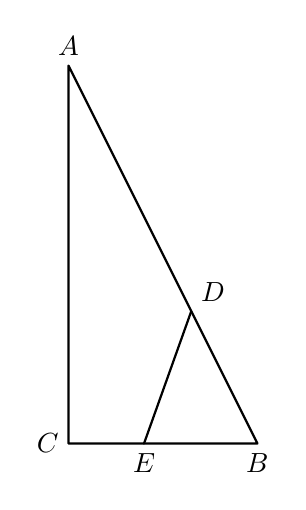
\begin{tikzpicture}[scale=1.2, line cap=round, line join=round]
    % --- 1. 定义核心顶点坐标 ---
    % 设定 C 为原点，根据图像比例设定 A 和 B 的位置
    \coordinate (C) at (0,0);
    \coordinate (A) at (0,4);
    \coordinate (B) at (2,0);
    
    % 定义斜边 AB 上的点 D (比例约在 AB 的 3/5 处)
    \coordinate (D) at ($(A)!0.65!(B)$);
    
    % 定义底边 CB 上的点 E (比例约在 CB 的中间)
    \coordinate (E) at ($(C)!0.4!(B)$);

    % --- 2. 绘制图形边框 ---
    % 绘制大三角形 ABC
    \draw[thick] (A) -- (B) -- (C) -- cycle;
    
    % 绘制内部线段 DE
    \draw[thick] (D) -- (E);

   

    % --- 3. 标注顶点文字 ---
    % anchor 用于微调文字相对于坐标点的方位
    \node[above] at (A) {$A$};
    \node[left]  at (C) {$C$};
    \node[below] at (B) {$B$};
    \node[above right] at (D) {$D$};
    \node[below] at (E) {$E$};

\end{tikzpicture}
\end{document}